\documentclass[reprint, amsmath, amssymb, aps]{revtex4-2}

\usepackage{graphicx}
\graphicspath{{./assets/figures/}}
\usepackage{dcolumn}
\usepackage{bm}
\usepackage{diagbox}
\usepackage[table]{xcolor}
\usepackage{hyperref}
\usepackage{comment}
\newcolumntype{L}{>{$}l<{$}} % math-mode version of "l" column type
\usepackage{float} % To fix location of tables with H
\usepackage[ruled,vlined]{algorithm2e}
\usepackage{braket}
\usepackage{amsthm}
\usepackage{cleveref}
\usepackage{mathtools}
\usepackage{listings} % to add python code

\newtheorem{definition}{Definition}
\newtheorem{prop}{Proposition}
\DeclareMathOperator{\tr}{Tr}

\begin{document}

\preprint{}

\title{Simulating Quantum Drude Oscillators on a photonic quantum computer}
%\thanks{}

\author{Matthieu Sarkis}
\email{matthieu.sarkis@uni.lu}
\affiliation{
Department of Physics and Materials Science\\ University of Luxembourg, L-1511, Luxembourg City, Luxembourg.
}

\author{}
\email{}
\affiliation{
}

%\collaboration{}%\noaffiliation

\date{\today}

\begin{abstract}
%\begin{description}
%\item[Usage]
%Secondary publications and information retrieval purposes.
%\item[Structure]
%You may use the \texttt{description} environment to structure your abstract;
%use the optional argument of the \verb+\item+ command to give the category of each item.
%\end{description}
\end{abstract}

%\keywords{Suggested keywords}%Use showkeys class option if keyword
                              %display desired
\maketitle

%\tableofcontents

\section{Introduction}

    Dispersion forces, also known as van der Waals (vdW) forces originate from the electromagnetic interaction between electrically neutral atoms or molecules which do not have permanent electric moments \cite{margenau2013theory,kaplan2006intermolecular,stone2013theory,hirschfelder2009intermolecular}. They are ever-present long-range forces between atoms or molecules arising from the zero-point fluctuations of the quantum electromagnetic field \cite{casimir1948influence,buhmann2013dispersion,buhmann2007dispersion,compagno1995atom,passante2018dispersion}. Their importance can be appreciated on both macro- and micro-scales; for instance, the first macroscopic signature of dispersion forces is the well-known correction to the equation of state of an ideal gas that led to the van der Waals equation \cite{milonni2013quantum}. Moreover, dispersion forces also influence the structure of liquids and solids such as the anomalies of water \cite{schmid2001recent} as well as the macroscopic properties of macromolecules such as their structure \cite{hoja2019reliable}, stability \cite{hoja2018first,mortazavi2018structure}, dynamics \cite{stohr2019quantum,reilly2014role,galante2021anisotropic}, and electric \cite{kleshchonok2018tailoring} and optical \cite{ambrosetti2022optical} responses. The most natural framework for the investigation of the response of matter subjected to such forces is quantum electrodynamics \cite{cohen1997photons,cohen1998atom,bookpreparata,salam2009molecular,craig1998t}. However, as widely shown in the literature, the inclusion of vdW dispersion interactions can be done by means of many-body methods \cite{richardson1975dispersion,mahanty1973dispersion,woods2016materials,tkatchenko2015current,ren2012random,harl2009accurate,dobson2012calculation,parsegian2005van}. Dispersion vdW interactions are often represented within the Lennard-Jones approach, namely, through a pairwise two-body interatomic potential \cite{becke2006simple,becke2006exchange,grimme2010consistent,grimme2006semiempirical,tkatchenko2012accurate,massa2021many} of the form $C_{6}/R^{6}$ (where $R$ is the interatomic distance and $C_6$ a system-dependent constant). Among all the existing models in the literature, the many-body dispersion (MBD) framework has been undoubtedly proved to be an accurate approach \cite{tkatchenko2012accurate,ambrosetti2014long}. In the MBD framework, the drudonic response of valence drudons in atoms and molecules is supposed to be linear and this can be formally done through the introduction of the quantum Drude oscillator (QDO). A single QDO is coarse-grained quantum-mechanical model in which the properties of an atom are encompassed in a small number of parameters. The model consists in assimilating the atom to a point particle of mass $m$ and electric charge $-q$ attached to a fixed (infinite mass) center of charge $+q$ by a harmonic spring characterized by a frequency $\omega$. Molecules are then defined as a collection of QDOs in dipole-dipole interaction.
    For some specific choices of the matter system geometry, the quantum Hamiltonian can be exactly diagonalized. For instance, in a closed linear chain of molecules, one can analytically solve for the spectrum of the Hamiltonion \cite{doi:10.1063/1.1743992}. In the case of a general geometry, instead, one can solve for the London-van der Waals interaction energy through a perturbative approach \cite{doi:10.1063/1.1743991}.
    This simple model has been extensively used in various contexts, for instance in order to tackle the drudonic structure problem for isolated molecules, in particular long range interactions, as well as to study the impact of an ambient bath or of an external electric field on molecular properties \cite{Karimpour_2022, karimpour2021comprehensive}.
    Though simple, through a numerical treatment this system was shown to capture long-range phenomena in large biomolecular systems \cite{https://doi.org/10.48550/arxiv.2205.11549}. By construction, the MBD framework relies on the dipole approximation of the drudon–drudon Coulomb interaction leaving aside any contribution coming from high-order terms. In the literature, dispersion forces have been addressed mostly for atomic dimers and small systems, via multipolar generalizations of the pairwise second-order perturbative approaches \cite{massa2021beyond,massa2021many,becke2006simple,becke2006exchange}.
    In this Letter ...
    \textcolor{purple}{They did full coulomb FCI in \cite{sadhukhan2016quantum}}

    \begin{figure}
    \label{fig:qdos}
        %\hspace{1.25cm}
        %\begin{subfigure}
        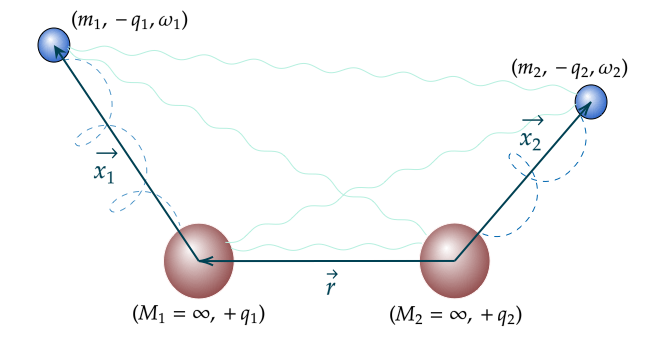
\includegraphics[scale=0.35]{figures/qdos.png}
        %\end{subfigure}
        \caption{a}
    \end{figure}


\section{Definition of the model}

    \subsection{Three-dimensional model}

        The Hamiltonian describing a system of $N$ Quantum Drude Oscillators in three dimensions is given by:
        \begin{equation}
        \label{eq:full_QDO_Hamiltonian}
            H=\sum_{i=1}^N\left[\frac{\bm{p} _i^2}{2m_i} + \frac{1}{2}m_i\omega_i^2\bm{x} _i^2\right] +\sum_{i<j}V_\text{Coul}\left(\bm{x} _i, \bm{x} _j\right)\,,
        \end{equation}
        with the Coulomb interaction receiving contributions from interacting drudon-drudon and drudon-nucleus pairs:
        \begin{equation}
        \label{eq:full_coulomb_potential}
        \begin{split}
            \frac{V_\text{Coul}\left(\bm{x} _i, \bm{x} _j\right)}{q_iq_j}=&\ \frac{1}{r_{ij}} - \frac{1}{|\bm{r}_{ij}
            + \bm{x} _i|} - \frac{1}{|\bm{r}_{ij}  - \bm{x} _j|} \\
            & + \frac{1}{|\bm{r}_{ij} - \bm{x} _j + \bm{x} _i|}\,.
        \end{split}
        \end{equation}
        The usual approach consists in solving the theory in the multipolar expansion framework, in which the potential can be expressed as a power series in the inverse distance separating the two centers:
        \begin{equation}
            V_\text{Coul}\left(\bm{x} _i, \bm{x} _j\right)= \sum_{n\geq 0} V_n\left(\bm{x} _i, \bm{x} _j\right)\,,
        \end{equation}
        with the following scaling behavior in terms of the distance between the centers:
        \begin{equation}
            V_n\left(\bm{x} _i, \bm{x} _j\right)\propto r_{ij}^{-n-3}\,.
        \end{equation}
        The potential $V_0$ corresponds then to the dipole-dipole interaction, and is at the core of the Many Body Dispersion (MBD) model. $V_1$ corresponds to the dipole-quadrupole interaction, and $V_2$ to the quadrupole-quadrupole and dipole-octupole interaction.

        One obvious limitation of the multipolar expansion is the lower bound it imposes on the interatomic distance. One can easily see that within the MBD (dipole-dipole) model by direct diagonalization of the quadratic Hamiltonian in terms of normal modes. In that case, one of the normal modes (the center of mass mode) develops a purely imaginary frequency at short range. Higher order physical effects are also neglected in the MBD model, motivating the study of the QDO model with full Coulomb interaction potential between its constituents.

        Let us define the following dimensionless position and momententum operators associated to QDO $i$:
        \begin{equation}
            \bm{X}_i := \sqrt{\frac{m_i\omega_i}{\hbar}}\,\bm{x}_i\,,\ \ \ \ \ \bm{P}_i := \frac{\bm{p}_i}{\sqrt{\hbar m_i\omega_i}}\,,
        \end{equation}
        in terms of which the Hamiltonian reads
        \begin{equation}
        \begin{split}
            H =&\ \sum_{i=1}^N\frac{\hbar\omega_i}{2}\left(\bm X_{i}^2 + \bm P_{i}^2\right) \\
            & + \sum_{i<j}V_\text{Coul}\left(\sqrt{\frac{\hbar}{m_i\omega_i}}\bm{X} _i, \sqrt{\frac{\hbar}{m_j\omega_j}}\bm{X} _j\right)\,.
        \end{split}
        \end{equation}
        One can define the $3N$ creation and annihilation operators
        \begin{equation}
            \bm a_{i} = \frac{\bm X_{i} + i\bm P_{i}}{\sqrt 2}\,,\ \ \ \ \ \bm a^\dagger_{i} = \frac{\bm X_{i} - i\bm P_{i}}{\sqrt 2}\,,
        \end{equation}
        in terms of which the Hamiltonian reads
        \begin{equation}
        \begin{split}
            H &= \sum_{i=1}^N\hbar\omega_i\left(\bm a_{i}^\dagger\cdot\bm a_{i} +\frac{3}{2}\right) \\
            & + \sum_{i<j}V_\text{Coul}\left(\sqrt{\frac{\hbar}{m_i\omega_i}}\frac{\bm a_i + \bm a_i^\dagger}{\sqrt 2}, \sqrt{\frac{\hbar}{m_j\omega_j}}\frac{\bm a_j + \bm a_j^\dagger}{\sqrt 2}\right)\,.
        \end{split}
        \end{equation}
        Let us from now on restrict the problem to a pair of QDOs ($N=2$) for concreteness, though the following developements carry to bigger systems. We denote by $d$ the interatomic distance.

    \subsection{One-dimensional case}

        In order to reduce the complexity of the problem, let us define one-dimensional instances of the QDO model as follows: we restrict the movement of the two drudons to be along a common axis (directed by a unit vector $\hat{\bm e}_\theta$) which form an angle $\theta\in[0,\pi/2]$ with respect to the vector $\bm r_{12}$ connecting the two nuclei. We therefore have a family of one-dimensional models which can be obtained from the full-fledged 3d model simply by setting to zero the contribution from the oscillator modes belonging to the plane perpendicular to $\hat{\bm e}_\theta$. Let us denote by $(X, P)$ the remaining position and momentum degree of freedoms. As limiting cases, we obtain models in which the drudons are constrained to move either in the direction parallel to the axis separating the two nuclei ($\theta=0$), or perpendicular to the latter ($\theta=\pi/2$). Those two models were studied in \cite{anderson2022coarse} in the dipole-dipole approximation. In that paper, the authors encode the states in the truncated Fock space of the system into the state of a set of qubits, and run VQE-type algorithms on IBQ quantum processors. However as we will see, the angle $\theta$ captures the competition between \textit{existence of binding} (for small $\theta$) and \textit{smoothness} (for large $\theta$), and interesting one-dimensional model actually sit at values of $\theta$ in the open segment $(0,\pi/2)$.

        In the case of a generic angle $\theta$ and interatomic distance, the one-dimensional Coulomb potential reads:
        \begin{equation}
        \begin{split}
            &\frac{V_\text{Coul}^{\theta, d}(x_1, x_2)}{q_1q_2} = \frac{1}{d} - \frac{1}{\sqrt{d^2+2d(\cos\theta) x_1+x_1^2}} \\
            &- \frac{1}{\sqrt{d^2-2d(\cos\theta) x_2+x_2^2}} \\
            &+\frac{1}{\sqrt{d^2 - 2d(\cos\theta) (x_2-x_1) + (x_2-x_1)^2}}\,.
        \end{split}
        \end{equation}
        We therefore have a family of Hamiltonians parameterized by $(\theta, d)\in[0, \pi/2]\times\mathbb R_{>0}$:
        \begin{equation}
        \label{eq:finalHamiltonian}
        \begin{split}
            H_{\theta, d}=&\ \frac{\hbar\omega_1}{2}\left(P_1^2 + X_1^2\right) + \frac{\hbar\omega_2}{2}\left(P_2^2 + X_2^2\right)\\
            &+V_\text{Coul}^{\theta, d}\left(\sqrt{\frac{\hbar}{m_1\omega_1}}X_1, \sqrt{\frac{\hbar}{m_2\omega_2}}X_2\right)\,.
        \end{split}
        \end{equation}
        Alternatively, in terms of creation and annihilation operators, one has
        \begin{equation}
        \begin{split}
            H_{\theta, d} &= \hbar\omega_1\left( a_{1}^\dagger a_{1} +\frac{1}{2}\right) + \hbar\omega_2\left(a_{2}^\dagger a_{2} +\frac{1}{2}\right) \\
            & + V_\text{Coul}^{\theta, d}\left(\sqrt{\frac{\hbar}{m_1\omega_1}}\frac{a_1 + a_1^\dagger}{\sqrt 2}, \sqrt{\frac{\hbar}{m_2\omega_2}}\frac{a_2 + a_2^\dagger}{\sqrt 2}\right)\,.
        \end{split}
        \end{equation}
        For the simulation, we set $\hbar=1$ as well as $m_i=q_i=\omega_i=1$ for both QDOs.

\section{Photonic circuit and Variational Algorithm}

    The main point of this letter is to probe the very natural idea that photonic-based continuous variable quantum hardware should be perfectly suited to simulate bosonic degrees of freedom. The simplest example one can come up with is a finite collection of interacting bosonic harmonic oscillators, which is precisely the case for the Quantum Drude Oscillator model. Another application is the computation of correlation functions of bosonic quantum fields on a lattice, for which an exponential speedup can be achieved with respect to standard methods \cite{marshall2015quantum}.

    From a molecular physics and long-range intermolecular perspective, we are mainly interested in knowing the ground state of the system (\ref{eq:finalHamiltonian}). Among the various approaches, the mixed quantum-classical variational algorithms were shown to be particularly efficient at capturing the properties of potentially complicated quantum states. In the spirit of \cite{killoran2019continuous, arrazola2019machine}, we apply a continuous-variable version of the variational quantum eigensolver algorithm to extract the ground state of the QDO system. The ground state is obtained by optimizing the parameters of a parameterized optical circuit composed of linear multi-modes gates (two-mode beamsplitters and rotation gates), Gaussian gates (single-mode squeezing and displacement gates), as well as non-Gaussian gates (Kerr gates) implementing non-linearity.

    Overall, denoting by $\omega$ the set of all parameters, the circuit implements a unitary $U(\omega)$ acting on an input reference state that we simply take to be the Fock vacuum state $|0\rangle$. The state prepared by the circuit is therefore given by
    \begin{equation}
        |\psi(\omega)\rangle = U(\omega)|0\rangle\,.
    \end{equation}

    Once the ansatz state $|\psi(\omega)\rangle$ has been produced, one extracts the value of the energy in that state, given by
    \begin{equation}
        \langle\psi(\omega)|H|\psi(\omega)\rangle\,.
    \end{equation}
    Let us denote expectations in the state $|\psi(\omega)\rangle$ by angular brackets $\langle\cdot\rangle$.
    To be specific, let us take the model $H$, and let us denote by angular brackets the expectation in state $|\psi(\omega)\rangle$. One has
    \begin{equation}
    \label{eq:loss}
    \begin{split}
        \langle H\rangle =&\ \hbar\omega_1\left(\langle a_{1}^\dagger a_{1}\rangle+\frac{1}{2}\right)+\hbar\omega_2\left(\langle a_{2}^\dagger a_{2}\rangle+\frac{1}{2}\right)\\
        &+ \left\langle V_\text{Coul}^{\theta, d}\left(\sqrt{\frac{\hbar}{m_1\omega_1}} X_1, \sqrt{\frac{\hbar}{m_2\omega_2}} X_2\right)\right\rangle
    \end{split}
    \end{equation}
    by linearity of the expectation. On the second line one has to compute an expression of the form $\langle f(X_1, X_2)\rangle$. One therefore needs to extract the joint statistics of the position quadratures by preparation and measurements of the state $|\psi(\omega)\rangle$ in the quadrature basis, as summarized in alg. (\ref{alg:statistics_computation}). Once the joint probability density $\rho$ of $(X_1, X_2)$ in the state $|\psi(\omega)\rangle$ is known, one can compute
    \begin{equation}
        \langle f(X_1, X_2)\rangle = \int_{\mathbb R^{6}}f(x_1, x_2)\rho(x_1, x_2)\,\text{d}x_1\text{d}x_2\,,
    \end{equation}
    where the integral above should be understood a finite sum over a sufficiently refined grid in the position quadratures plane.
    Let us note that alternatively, the simulator of Strawberry Fields actually provides direct access to the output statevector expressed in the Fock basis:
    \begin{equation}
        |\psi(\omega)\rangle = \sum_{n_1,n_2=0}^\infty \alpha_{n_1n_2}(\omega)|n_1\rangle\otimes|n_2\rangle\,.
    \end{equation}
    The amplitude of a specific pair of the quadratures $(X_1, X_2)$ is then given by:
    \begin{equation}
        \langle X_1,X_2|\psi(\omega)\rangle = \sum_{n_1,n_2=0}^\infty \alpha_{n_1n_2}(\omega)\prod_{i=1}^{2}\frac{e^{-\frac{X_i^2}{2}}H_{n_i}(X_i)}{\sqrt{\pi^{1/2}2^{n_i}n_i!}}\,,
    \end{equation}
    in terms of the Hermite polynomials. The joint law of the quadratures in the state $|\psi\rangle$ is therefore given by
    \begin{equation}
        \rho(X_1,X_{2}) = \left|\langle X_1,X_2|\psi(\omega)\rangle\right|^2\,.
    \end{equation}
    After extracting as well the mean photon numbers $\langle n_1\rangle$ and $\langle n_2\rangle$, one obtains $\langle H\rangle$.

    We then define the cost function
    \begin{equation}
    \label{eq:definition_cost}
        \mathcal C(\omega) := \langle\psi(\omega)|H|\psi(\omega)\rangle\,,
    \end{equation}
    and update the parameters $\omega$ of the optical circuit in order to minimize that cost. This is summarized in alg. (\ref{alg:training})

    \begin{algorithm}
        \caption{Extract distribution of position quadratures}\label{alg:statistics_computation}
            \textbf{Parameters:} statevector $|\psi\rangle$, finite subset $\mathcal {G}\in\mathbb R$, shots $M\in\mathbb N$

            \KwResult{Probability distribution of $(X_1, X_2)$ in state $|\psi\rangle$ discretized over the grid $\mathcal G\times\mathcal G$}\

            \For{$m=1$ to $|\mathcal G|$}{
                Initialize $N_m \gets 0$;
            }
            \For{$j=1$ to $M$}{
            Measure the state $|\psi\rangle$ in the discretized position quadratures basis, obtain the eigenvalue $o_m$, set $N_m\gets N_m+1$\;
            }
            \For{$m=1$ to $|\mathcal G|$}{
                Normalize $N_m \gets N_m / M$;
            }
            \textbf{return} $\{N_m\}_{m=1}^M$.
    \end{algorithm}



    \begin{algorithm}
        \caption{Training of the parameterized photonic circuit}\label{alg:training}
        \textbf{Parameters:} Model $(\theta, d)$, $N_\text{steps}\in\mathbb N$, initial circuit parameters $\omega_0\in\mathbb R^K$, learning rate $\eta\in\mathbb R_+$

        \KwResult{Optimized hyperparameters $\omega\in\mathbb R^K$}\

        Initialize hyperparameters $\omega \gets \omega_0$\;
        \For{$i=1$ to $N_\text{steps}$}{
        Compute the loss $\mathcal C$ according to eq. (\ref{eq:definition_cost})\;
        Compute the gradient $\nabla_\omega\mathcal C$ with the shift rule\;
            Update the parameters $\omega \gets \omega - \eta\nabla_\omega\mathcal C$\;
        \textbf{end for}
        }
        \textbf{return} $\omega$.
    \end{algorithm}

\section{Results and interpretation}

    We gather here the results of the simulations. We focus on the case of 2 QDOs. In particular we plot the profile of the binding energy as a function of the distance between the two nuclei. The binding energy is simply defined as the ground state energy of the interacting system to which one substract the ground state energy of the uninteracting system, namely that of a pair of free harmonic oscillators in this Drude model.

\subsection{Binding energy curve}

    \textcolor{purple}{
    \begin{itemize}
        \item Morse fit
        \item Quality of Morse fit
        \item Smoothness vs. existence of binding
    \end{itemize}
    }

    \begin{figure}[H]
    \label{fig:binding}
        %\hspace{1.25cm}
        %\begin{subfigure}
        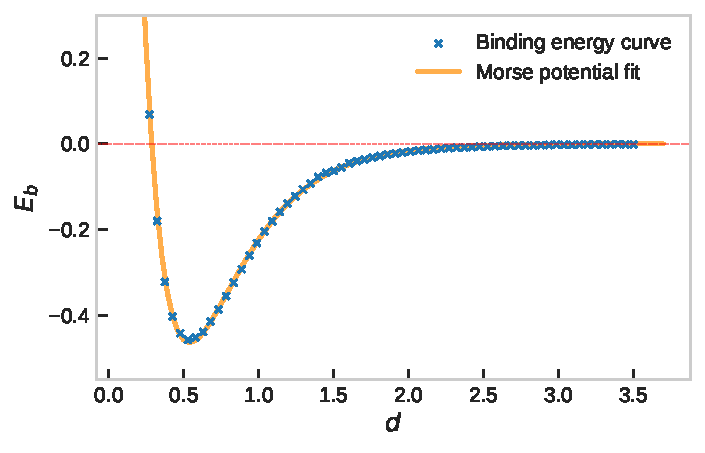
\includegraphics[scale=0.7]{figures/binding.pdf}
        %\end{subfigure}
        \caption{Binding curve for three differents values of the angle $\theta$. The larger the angle, the smoother the binding curve from the point of view of the Morse fit quality. However the bound state disappear for large $\theta$.}
    \end{figure}

\subsection{Ground state wavefunction}

    \begin{figure*}
    \label{fig:wigners_joint}
        %\hspace{1.25cm}
        %\begin{subfigure}
        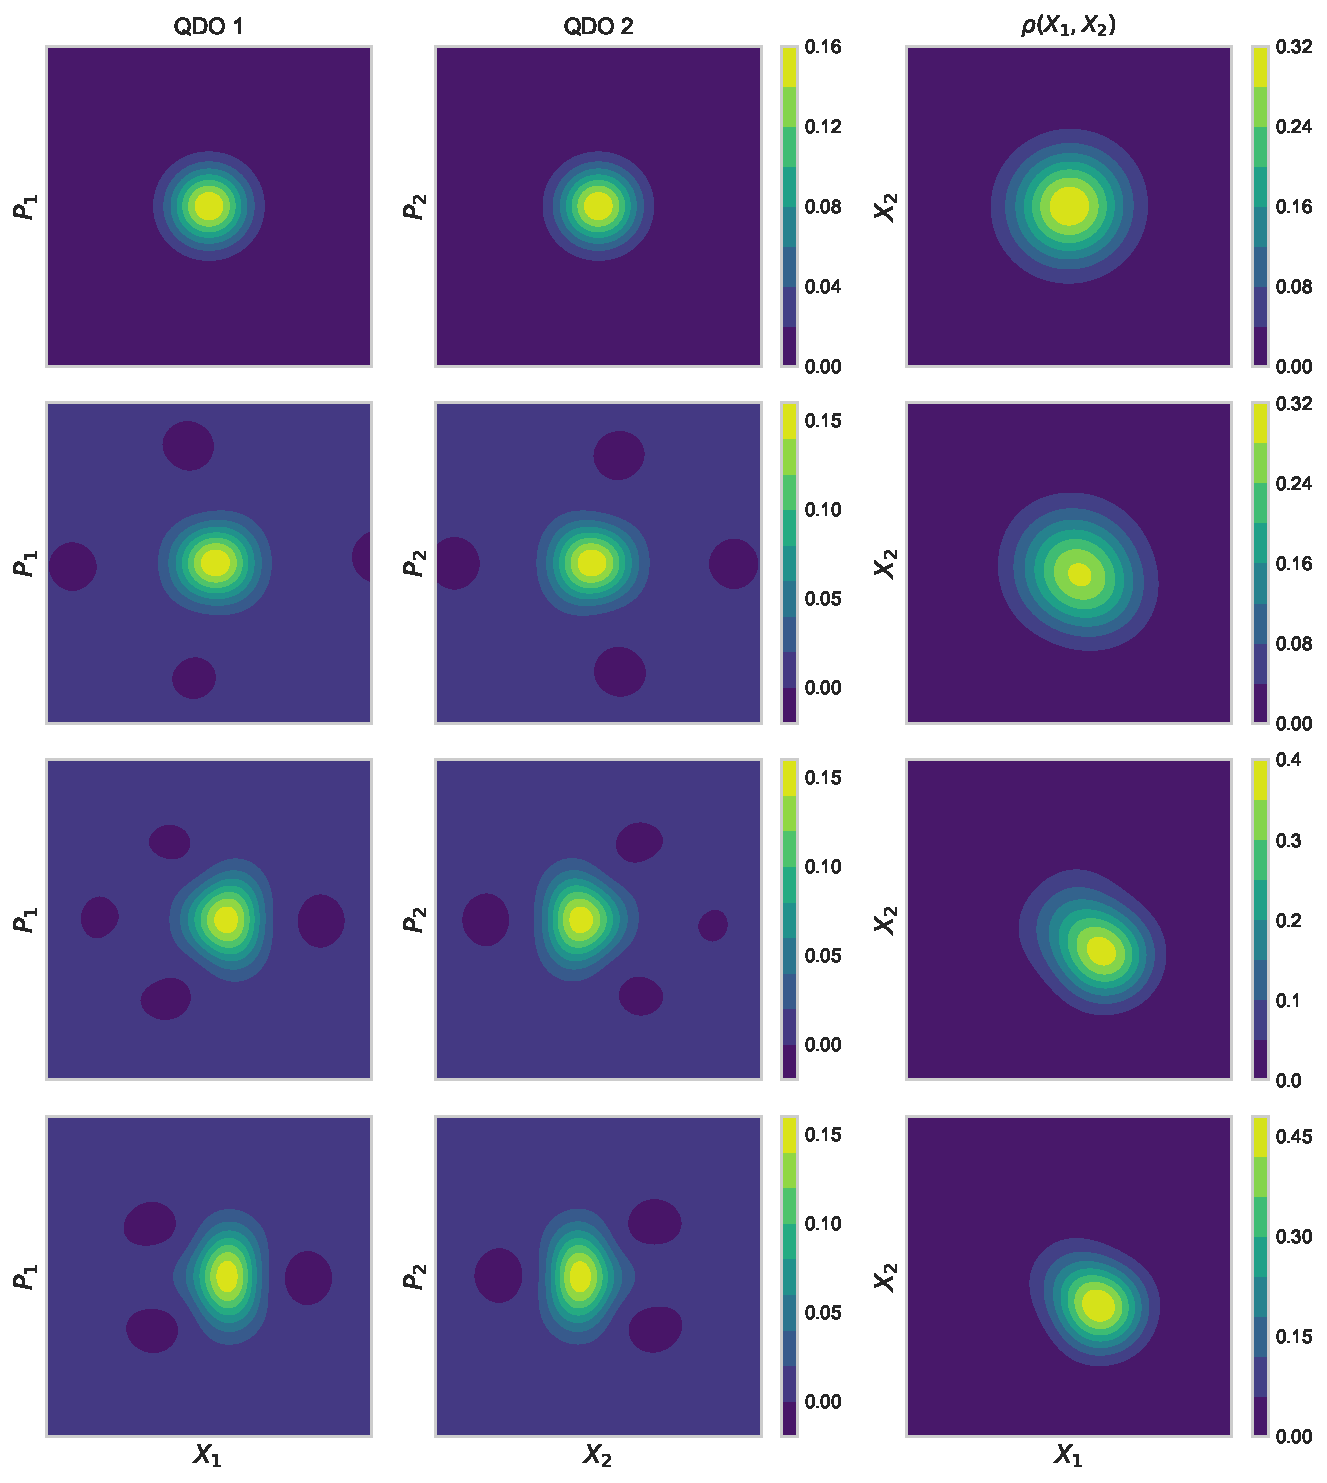
\includegraphics[scale=0.75]{figures/wigners_joint.pdf}
        %\end{subfigure}
        \caption{a}
    \end{figure*}

\subsection{Entanglement entropy and position quadratures correlation}

    Let us give the expression of the partial densitity matrix associated to $\text{QDO}_1$. The total state of the system, we recall, is expressed in the Fock basis as the pure state:
    \begin{equation}
        |\psi\rangle = \sum_{n_1,n_{2}=0}^\infty \alpha_{n_1n_2}|n_1\rangle\otimes|n_2\rangle\,.
    \end{equation}
    This state is directly accessible when using the simulator, and can be obtained on a genuine hardware by state tomography techniques \cite{Lvovsky:2009zz}. Given the state, the density matrix of the system is simply given by:
    \begin{equation*}
        \rho = \sum_{\substack{n_1,n_2 \\ m_1,m_2}} \alpha^*_{m_1m_2}\alpha_{n_1n_2}|n_1\rangle\langle m_1|\otimes|n_2\rangle\langle m_2|\,.
    \end{equation*}
    The partial trace associated to $\text{QDO}_1$ is therefore given by:
    \begin{equation}
        \rho_1 = \sum_{n, m, l} \alpha^*_{ml}\alpha_{nl}\,|n\rangle\langle m|\,.
    \end{equation}
    Since the state of the total system is pure, the von Neumann entropy of the total density matrix is zero. QDO 2 can then be interpreted as purifying the system composed solely of QDO 1. The two QDOs therefore have identical von Neumann entropy $S(\rho_1)$, the entanglement entropy. The quantum mutual information of the system is therefore given by
    \begin{equation}
        I(1:2) = S(\rho_1) + S(\rho_2) - S(\rho) = 2S(\rho_1) \,,
    \end{equation}
    with the von Neumann entropy being defined as
    \begin{equation}
        S(\rho) = -\text{Tr}\left[\rho\log\rho\right]\,.
    \end{equation}
    Another intersting quantity to consider is the quantum correlation between the the position quadrature of the two QDOs. Denoting again by angular brackets the expectation of an observable in the ground state, the correlation coefficient is defined by:
    \begin{equation}
        C(X_1, X_2) = \frac{\langle X_1X_2\rangle - \langle X_1\rangle\langle X_2\rangle}{\sqrt{\langle X_1^2\rangle - \langle X_1\rangle^2}\sqrt{\langle X_2^2\rangle - \langle X_2\rangle^2}}\,.
    \end{equation}
    The profile of the quantum mutual information as a function of the interatomic distance is provided in fig. (...)




    \begin{figure}
    \label{fig:entropy_correlation}
        %\hspace{1.25cm}
        %\begin{subfigure}
        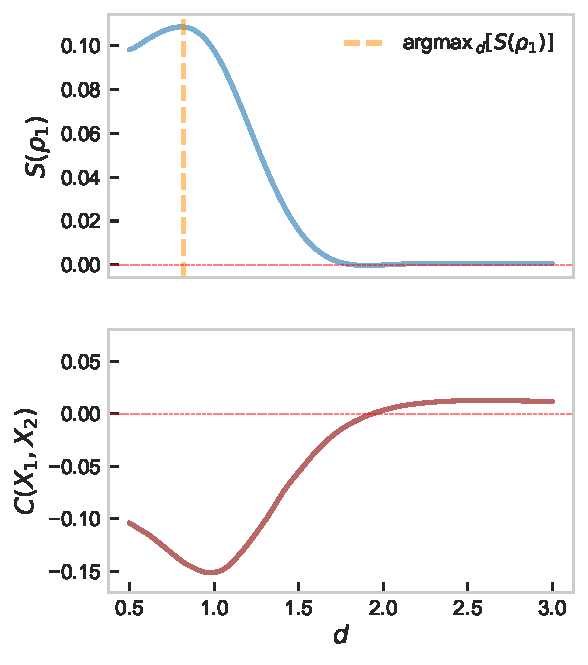
\includegraphics[scale=0.9]{figures/entropy_correlation.pdf}
        %\end{subfigure}
        \caption{\textbf{On the top.} Entanglement entropy vs. interatomic distance. \textbf{On the bottom.} Position quadratures correlation coefficient vs. interatomic distance. Both curves correspond to an angle $\theta=0.58$.}
    \end{figure}

    \begin{figure}
    \label{fig:morse_quality}
        %\hspace{1.25cm}
        %\begin{subfigure}
        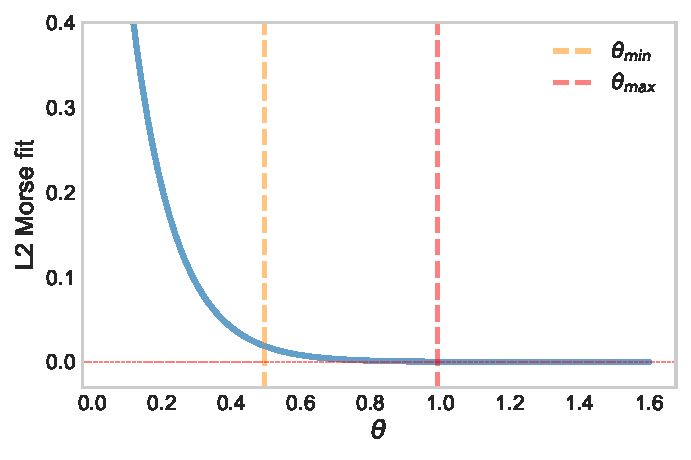
\includegraphics[scale=0.75]{figures/morse_quality.pdf}
        %\end{subfigure}
        \caption{}
    \end{figure}






\section{Conclusion}

\begin{acknowledgments}

    We would like to thank Dahvyd Wing and Kyunghoon Han for important discussions.

\end{acknowledgments}

\section*{Code Availability}

The reader will find an open source python code accompanying this paper at \href{https://github.com/MatthieuSarkis/qdo}{github repository}.

\appendix

\nocite{*}
\bibliographystyle{IEEEtran}
\bibliography{bibliography}

\end{document}


%%%%%%%%%%%%%%%%%%%%%%%%%%%%%%%%%%%%%%%%%%%%%%%%%%%%
%%%%%%%%%%% UNUSED CODE %%%%%%%%%%%%%%%%%%%%%%%%%%%%
%%%%%%%%%%%%%%%%%%%%%%%%%%%%%%%%%%%%%%%%%%%%%%%%%%%%


Let us give here the expression for the multipolar potential up to quartic order:
        \begin{align}
            V_0(\bm{x} _i, \bm{x} _j) &= q_iq_j\frac{x_ix_j + y_iy_j - z_iz_j}{r_{ij}^3}\\
            V_1(\bm{x} _i, \bm{x} _j) &= \frac{q_iq_j}{2r_{ij}^4}\big(-3  x_i ^2  z_j -6  x_i   x_j   z_i +6  x_i   x_j   z_j +3  x_j ^2  z_i\nonumber\\
            & -3  y_i ^2  z_j -6  y_i   y_j   z_i +6  y_i   y_j   z_j +3  y_j ^2  z_i\nonumber\\
            & +6  z_i ^2  z_j -6  z_i   z_j ^2\big)\\
            V_2(\bm{x} _i, \bm{x} _j) &= \frac{q_iq_j}{2 r_{ij}^4}\big(-6  x_i ^3  x_j +9  x_i ^2  x_j ^2-6  x_i ^2  y_i   y_j +3  x_i ^2  y_j ^2\nonumber\\
            &+24  x_i ^2  z_i   z_j -12  x_i ^2  z_j ^2-6  x_i   x_j ^3-6  x_i   x_j   y_i ^2\nonumber\\
            &+12  x_i   x_j   y_i   y_j -6  x_i   x_j   y_j ^2+24  x_i   x_j   z_i ^2\nonumber\\
            &-48  x_i   x_j   z_i   z_j +24  x_i   x_j   z_j ^2+3  x_j ^2  y_i ^2-6  x_j ^2  y_i   y_j \nonumber\\
            &-12  x_j ^2  z_i ^2+24  x_j ^2  z_i   z_j -6  y_i ^3  y_j +9  y_i ^2  y_j ^2\nonumber\\
            &+24  y_i ^2  z_i   z_j -12  y_i ^2  z_j ^2-6  y_i   y_j ^3+24  y_i   y_j   z_i ^2\nonumber\\
            &-48  y_i   y_j   z_i   z_j +24  y_i   y_j   z_j ^2-12  y_j ^2  z_i ^2+24  y_j ^2  z_i   z_j \nonumber\\
            &-16  z_i ^3  z_j +24  z_i ^2  z_j ^2-16  z_i   z_j ^3\big)
        \end{align}



        \begin{equation}
            \begin{split}
                &V_0(x_i, x_j) = q_iq_j\frac{x_ix_j}{r_{ij}^3}\times\\
                &\times\begin{cases}
                    1-3\cos^2\theta, & \text{generic case} \\
                    -2, & \text{parallel case} \\
                    1, & \text{perpendicular case} \\
                    -\frac{1}{2}, & \text{oblique case} \\
                    -2-6\epsilon, & \text{regularized case}
                \end{cases}
            \end{split}
            \end{equation}
            The next terms in the multipolar expansion are:
            \begin{equation}
            \begin{split}
                &V_1(x_i, x_j) = q_iq_j\frac{x_ix_j(x_i-x_j)}{r_{ij}^4}\times\\
                &\times\begin{cases}
                    \frac{3\cos\theta(-3+5\cos^2\theta)}{2}, & \text{generic case} \\
                    3, & \text{parallel case} \\
                    0, & \text{perpendicular case} \\
                    -\frac{3}{4\sqrt 2}, & \text{oblique case} \\
                    3+18\epsilon, & \text{regularized case}
                \end{cases}
            \end{split}
            \end{equation}
            \begin{equation}
                \begin{split}
                    &V_2(x_i, x_j) = q_iq_j\frac{x_ix_j(2x_i^2-3x_ix_j+2x_j^2)}{r_{ij}^5}\times\\
                    &\times
                    \begin{cases}
                        -\frac{3-30\cos^2\theta+35\cos^4\theta}{4}, & \text{generic case} \\
                        -2, & \text{parallel case} \\
                        -\frac{3}{4}, & \text{perpendicular case} \\
                        \frac{13}{16}, & \text{oblique case} \\
                        -2-20\epsilon, & \text{regularized case}
                    \end{cases}
                \end{split}
            \end{equation}

            \subsection{12 different models}

            For the simulation, we will restrict the system to two QDOs. Depending on the space dimensionality (1d oblique, 1d parallel, 1d perpendicular, 3d) and the choice of potential (quadratic, quartic, Coulomb), we therefore have 12 models to try and study, gathered in table (\ref{tab:models}).
            \begin{table}[ht!]
            \caption{\label{tab:models} The twelve models}
            \begin{ruledtabular}
            \begin{tabular}{c|cccc}
                \diagbox[height=1.8\line]{\textsc{pot}}{\textsc{dim}}& 1d oblique & 1d parallel & 1d perpendicular & 3d \\
                \hline\\[-0.95em]
                \textsc{quad} & $H_{(1,0)}$ & $H_{(1,1)}$ & $H_{(1,2)}$ & $H_{(1,3)}$ \\
                \textsc{quart} & $H_{(2,0)}$ & $H_{(2,1)}$ & $H_{(2,2)}$ & $H_{(2,3)}$\\
                \textsc{Coulomb} & $H_{(3,0)}$ & $H_{(3,1)}$ & $H_{(3,2)}$ & $H$ \\
            \end{tabular}
            \end{ruledtabular}
            \end{table}

            The space regularized model Coulomb potential reads
            \begin{equation}
            \begin{split}
                &\frac{V_\text{Coul}^\epsilon(x_i, x_j)}{q_iq_j} = \frac{1}{r_{ij}} - \frac{1}{\sqrt{r_{ij}^2+2r_{ij}(1+\epsilon) x_i+x_i^2}} \\
                &- \frac{1}{\sqrt{r_{ij}^2-2r_{ij}(1+\epsilon) x_j+x_j^2}} \\
                &+\frac{1}{\sqrt{r_{ij}^2 - 2r_{ij}(1+\epsilon) (x_j-x_i) + (x_j-x_i)^2}}\,.
            \end{split}
            \end{equation}

            In terms of components, the full Coulomb potential reads:
            \begin{equation}
            \mathclap{
            \begin{split}
                &\frac{V_\text{Coul}(\bm{x} _i, \bm{x} _j)}{q_iq_j} = \frac{1}{r_{ij}} - \frac{1}{\sqrt{r_{ij}^2 + x_i^2+y_i^2+z_i^2+2rz_i}} \\
                &- \frac{1}{\sqrt{r_{ij}^2 + x_j^2+y_j^2+z_j^2-2r_{ij}z_j}} \\
                &+\frac{1}{\sqrt{r_{ij}^2 + (x_j-x_i)^2+(y_j-y_i)^2+(z_j-z_i)^2-2r_{ij}(z_j-z_i)}}
            \end{split}
            }
            \end{equation}

            For the full Coulomb potential, assuming that the drudons are constrained to move along an axis, we get the following expressions:
            \begin{equation}
            \begin{split}
                \frac{V_\text{Coul}^\perp(x_1, x_2)}{q_1q_2} = &\ \frac{1}{r_{12}} - \frac{1}{\sqrt{r_{12}^2+x_1^2}} - \frac{1}{\sqrt{r_{12}^2+x_2^2}} \\
                &+\frac{1}{\sqrt{r_{12}^2 + (x_2-x_1)^2}}
            \end{split}
            \end{equation}
            in the case where the drudons move perpendicular to the axis joining the two nuclei, and
            \begin{equation*}
            \mathclap{
                \frac{V_\text{Coul}^{||}(x_1, x_2)}{q_1q_2} = \frac{1}{r_{12}} - \frac{1}{|r_{12}+x_1|} - \frac{1}{|r_{12}-x_2|} + \frac{1}{|r_{12}+x_1-x_2|}
            }
            \end{equation*}
            in the case where they move parallel to the latter.


            \begin{equation}
                |\psi(\omega)\rangle = \sum_{n_1,\dots,n_{2K}=0}^\infty \alpha_{n_1\dots n_{2K}}|n_1\rangle\otimes\dots\otimes|n_{2K}\rangle\,.
            \end{equation}
            The modes labeled by $(n_1,\dots,n_K)$ correspond to $\text{QDO}_1$, while the modes $(n_{K+1},\dots,n_{2K})$ are attached to $\text{QDO}_2$.
            The amplitude of a specific tuple of the quadratures $(X_1,\dots, X_{K})$ is therefore given by:
            \begin{equation*}
            \mathclap{
                \langle X_1,\dots,X_{2K}|\psi\rangle = \sum_{n_1,\dots,n_{2K}=0}^\infty \alpha_{n_1\dots n_{2K}}\prod_{i=1}^{2K}\frac{e^{-\sum_{i=1}^{2K}\frac{X_i^2}{2}}H_{n_i}(X_i)}{\sqrt{\pi^{1/2}2^{n_i}n_i!}}\,,
            }
            \end{equation*}
            in terms of the Hermite polynomials. The joint law of the quadratures in the state $|\psi\rangle$ is therefore given by
            \begin{equation}
            \begin{split}
                \rho(X_1,\dots,X_{2K}) &= \sum_{\substack{n_1,\dots,n_{2K} \\ m_1,\dots,m_{2K}}} \alpha_{n_1\dots n_{2K}}\alpha^*_{m_1\dots m_{2K}}\\
                &\times\prod_{i=1}^{2K}\frac{e^{-X_i^2}H_{n_i}(X_i)H_{m_i}(X_i)}{\sqrt{\pi^{1/2}2^{n_i}n_i!}\sqrt{\pi^{1/2}2^{m_i}m_i!}}
            \end{split}
            \end{equation}
            After extracting as well the mean photon numbers $\langle n_{i,\alpha}\rangle$, one obtains $\langle H\rangle$.

            \begin{algorithm}
                \caption{Computation of the loss}\label{alg:loss_computation}
                    \textbf{Parameters:} $M\in\mathbb N$

                    \KwResult{Value of the loss $\mathcal C$}\

                    Initialize $\mathcal C \gets 0$\;
                    Get the position quadratures distribution with alg. (\ref{alg:statistics_computation})\;
                    Get the photon numbers distribution with alg. (\ref{alg:statistics_computation})\;
                    Compute the loss $\mathcal C$ using eq. (\ref{eq:loss})\;
                    \textbf{return} $\mathcal C$.
            \end{algorithm}

            \begin{equation}
                |\psi\rangle = \sum_{n_1,\dots,n_{2K}=0}^\infty \alpha_{n_1\dots n_{2K}}|n_1\rangle\otimes\dots\otimes|n_{2K}\rangle\,,
            \end{equation}
            leading to the following expression for the density matrix:
            \begin{equation*}
            \mathclap{
                \rho = \sum_{\substack{n_1,\dots,n_{2K} \\ m_1,\dots,m_{2K}}} \alpha^*_{m_1\dots m_{2K}}\alpha_{n_1\dots n_{2K}}|n_1\rangle\langle m_1|\otimes\dots\otimes|n_{2K}\rangle\langle m_{2K}|\,.
            }
            \end{equation*}
            The partial trace associated to $\text{QDO}_1$ is therefore given by:
            \begin{equation}
            \begin{split}
                \rho_1 = \sum_{\substack{n_1,\dots,n_{K} \\ m_1,\dots,m_{K} \\ l_1,\dots,l_{K}}}& \alpha^*_{m_1\dots m_{K}l_1,\dots,l_{K}}\alpha_{n_1\dots n_{K}l_1,\dots,l_{K}}\\
                &|n_1\rangle\langle m_1|\otimes\dots\otimes|n_{K}\rangle\langle m_{K}|\,.
            \end{split}
            \end{equation}